\documentclass[11pt]{article}

% --- Packages ---
\usepackage[utf8]{inputenc}
\usepackage[T1]{fontenc}
\usepackage{times}
\usepackage{geometry}
\geometry{a4paper, margin=2cm}
\usepackage{multicol}
\usepackage{abstract}
\usepackage{graphicx}
\usepackage{booktabs}
\usepackage{amsmath}
\usepackage{hyperref}
\usepackage{natbib}
\usepackage{lineno}
\usepackage{caption}
\usepackage{float}
\usepackage{enumitem}
\usepackage{titlesec}
\usepackage{xcolor}
\usepackage{listings}

\lstdefinelanguage{json}{
    basicstyle=\ttfamily\small,
    numbers=left,
    numberstyle=\small,
    stepnumber=1,
    numbersep=8pt,
    showstringspaces=false,
    breaklines=true,
    frame=single,
    backgroundcolor=\color{gray!10},
    string=[s]{"}{"},
    stringstyle=\color{green!50!black},
    comment=[l]{//},
    morecomment=[s]{/*}{*/},
    commentstyle=\color{gray},
    keywordstyle=\color{blue},
    morekeywords={true,false,null}
}

% --- Title formatting ---
\titleformat{\section}{\normalfont\large\bfseries}{\thesection}{1em}{}
\titleformat{\subsection}{\normalfont\normalsize\bfseries}{\thesubsection}{1em}{}
\titleformat{\subsubsection}{\normalfont\normalsize\bfseries}{\thesubsubsection}{1em}{}

% --- Two-column abstract ---
\renewcommand{\abstractnamefont}{\normalfont\bfseries}
\renewcommand{\abstracttextfont}{\normalfont\small}

% --- Guidance command: renders in blue, easy to delete before submission ---
% To hide all guidance notes, change \guidancetrue to \guidancefalse
\newif\ifguidance
\guidancetrue
\newcommand{\guidance}[1]{\ifguidance\textcolor{blue}{\small\textit{[#1]}}\fi}

% --- Title ---
\title{\Large\textbf{Real-time Multiparty Disembodied-LLM Dialogue System for Education}}

\author{
  Mats Kroneberg and Gonzalo Larroya and Abdulsalam Umar and\\
  Terry Olampi and Arthur Ollivier and Afreen Begum\\
  \textit{Conversational Agents Course -- Final Report} \\
  Heriot-Watt University, Edinburgh, United Kingdom \\
  \texttt{\{mmk12, gl4003, ...\}@hw.ac.uk}
}

\date{}

\begin{document}

\maketitle



% ============================================================
% ABSTRACT (Part of 10-mark criterion)
% ============================================================
% MARKING CRITERION: "Abstract, Aims, Objectives and Project Description" [10 marks]
%   - Abstract succinctly describes the project
%   - Research aims of the project are clear

\begin{abstract}
\noindent
\guidance{%
  MARKING: This section contributes to the ``Abstract, Aims, Objectives and
  Project Description'' criterion (10 marks). The abstract must succinctly
  describe the project. Cover: (1) the problem/task addressed, (2) your
  approach and key components, (3) evaluation methods used, and (4) main
  findings. Keep to 100--200 words. The marker will check that research
  aims are immediately apparent from reading this.}

% Write your abstract here.


\end{abstract}



% --- Begin two-column layout ---
\begin{multicols}{2}
\raggedcolumns

\section{Introduction}
\label{sec:introduction}
% ============================================================
% MARKING CRITERION: "Abstract, Aims, Objectives and Project Description" [10 marks]
%   - Research aims of project are clear

%\guidance{%
%  MARKING: The introduction also contributes to the ``Aims, Objectives and
%  Project Description'' criterion (10 marks). Make the research aims and
%  objectives of the project unmistakably clear. The marker will look for:
%  (a) a well-motivated problem statement, (b) explicit research aims /
%  objectives, (c) a summary of the approach taken, and (d) a roadmap of
%  the report.}

\subsection{Problem Statement and Motivation}
While LLM-based educational agents offer high linguistic fluency, 
most existing systems rely on dyadic (one-on-one) text interactions that fail to capture the social dynamics of classroom learning. 
A key pedagogical gap lies in the absence of vicarious learning, the process where students gain knowledge by observing interactions between others. 
Passive learners often struggle to identify their own knowledge gaps, a problem exacerbated by the cognitive load of managing a dialogue. 
By moving away from text-only interfaces toward a triadic, real-time spoken "fictive dialogue", 
we can simulate a more natural and effective learning environment that triggers deeper reflection through agentic exchanges.

% Describe the broader context and why this problem matters.
% What gap or need does your work address?

\subsection{Research Aims and Objectives}
The primary aim of this project is to demonstrate how a multi-agent architecture can foster vicarious learning through autonomous student-teacher interactions.
The specific objectives are:
\begin{enumerate}[noitemsep, leftmargin=*]
  \item To develop a Teacher Agent capable of delivering structured, pedagogically sound content via a spoken channel.
  \item To implement an autonomous Student Agent that mimics human curiosity by interjecting with clarifying questions.
  \item To integrate low-latency speech technologies (Whisper STT and Chatterbox TTS) to manage a fluid triadic interaction.
  \item To evaluate the impact of a "synthetic peer" on user engagement and conceptual retention through controlled human testing.
\end{enumerate}

%\guidance{%
%  State your aims and objectives explicitly. Consider using a short
%  enumerated list so the marker can see them at a glance.}

% Example:
% The aims of this project are:
% \begin{enumerate}[noitemsep]
%   \item To implement ...
%   \item To evaluate ...
%   \item To investigate ...
% \end{enumerate}

\subsection{Experimental overview}

To demonstrate the effectiveness of our hypothesis, we conducted a user study comparing two pedagogical conditions: 
a standard dyadic interaction (Teacher-Human) and our proposed triadic fictive dialog (Teacher-Student-Human).

Participants are tasked with learning a specific topic through a spoken session in real-time. 
We measure learning gains through pre- and post-interaction assessments, while qualitative engagement is captured through subjective questionnaires. 
This setup allows us to isolate the impact of the Student Agent’s interjections on the user’s understanding and overall experience.


\section{Previous Work}
\label{sec:previous_work}
% ============================================================
% MARKING CRITERION: "Literature Review" [40 marks]


\subsection{Dialogue, Vicarious Learning, and Educational Conversational Agents}
\label{sec:background}

For nearly two decades, spoken dialogue systems (SDS) have been
investigated in educational contexts, particularly for intelligent
tutoring \citep{litman2004itspoke, pon-barry2004scot} and language
learning \citep{seneff-etal-2007-spoken, bibauw2019dialogue}, and more
recently as conversational agents powered by large language models
\citep{Sydorenko2025}. Dialogue has been demonstrated to be a more effective modality than plain
text for knowledge retention \citep{ginns2013designing}, and merely
\emph{overhearing} dialogue between agents has itself been shown to
support learning better than listening to a monologue \citep{vicarious_learning}.

This phenomenon, coined vicarious learning, has been investigated
through "fictive dialogues": semi-scripted exchanges between virtual
agents generated from a source text, where the learner is a passive
listener rather than an active participant \citep{piwek2007t2d}.
\citet{fictive_dialogs} extend the paradigm to a classroom
language-learning Educational Conversational Agent (ECA) that
alternates between teacher and peer roles. They find that more
scripted agent and human-confederate exchanges improve comprehension, whereas
direct agent-to-learner questioning degrades it.
The multi-party configurations needed for designing such agentic
conversations remain a known open challenge for current systems
\citep{aylett2023you, skantze2021turntaking}, primarily because
realtime end-of-turn prediction, addressee detection and overlap
handling all degrade sharply once the dyadic speak/wait assumption
is dropped.

\subsection{LLM-based and Multi-Agent Tutors}
\label{sec:llm_tutors}

A recent systematic review of 36 educational chatbots finds that
teaching agents and peer agents together dominate deployed roles
\citep{kuhail2023interacting} --- a decomposition that maps directly
onto the teacher and question-asking student configuration the
present system adopts. Empirical evidence on the pedagogical effects
of the LLM-based variants of such systems, however, is only
beginning to accumulate. \citet{SpangenbergerPia2026CwaL}
evaluate chat-based conversation with an LLM in education for
sustainable development ($N=122$) and find that LLM chat engages both
affective and cognitive processes relevant to
learning, and yields knowledge gains comparable to reading the same
material as text. This establishes LLM chat as a viable instructional
medium rather than a pedagogical novelty. What unstructured dyadic
LLM chats still lack, however, is the curricular sequencing and
student modelling that drove the gains reported for earlier
conversational intelligent tutoring systems such as AutoTutor, which
was shown to produce learning gains on par with human tutors
\citep{graesser2016autotutor}.

A recent architectural response is to recover that pedagogical
structure by composing several specialised LLM agents rather than
relying on a single chatbot or hand-authored dialogue policy. The
WikiHowAgent system of \citet{pei-etal-2025conversational}
instantiates teacher, student, interaction-manager and evaluator
agents at scale; \citet{shi-etal-2025-educationq} apply a similar
triadic teacher--student--evaluator framework (EducationQ) to
benchmark teaching ability across 14 LLMs. Both systems place no
human in the interactive loop --- the human enters only as a
post-hoc judge. The present work adopts the same multi-agent
decomposition but narrows the student agent to a question-asking
role whose purpose is to elicit teacher exposition that a human
learner overhears or joins, over a realtime spoken channel rather
than text.

\subsection{Speech Interfaces for Educational Agents}
\label{sec:speech_interfaces}

The few LLM-era ECAs that do operate in the spoken modality
typically pair their dialogue manager with cloud-based speech I/O:
\citet{fictive_dialogs}, for instance, integrate Deepgram's hosted
ASR and TTS synthesis into a RASA dialogue agent.
\citet{Sydorenko2025} identify recognition error and end-to-end
latency as the two persistent bottlenecks for spoken educational
agents --- a concern echoed in the realtime turn-taking literature
\citep{skantze2021turntaking}. The present system adopts the same
two-component STT/TTS split but runs both locally (Whisper for STT,
Chatterbox for TTS), trading on-device compute for lower latency
and no external dependency in the realtime loop.

\subsection{Summary}
\label{sec:prev_work_summary}

Our system sits at the intersection of three traditions: the
dialogue-based intelligent tutoring tradition
\citep{litman2004itspoke, pon-barry2004scot} with its spoken,
pedagogically-structured interaction; the recent LLM-based tutor
wave \citep{SpangenbergerPia2026CwaL, pei-etal-2025conversational},
which contributes fluent generation and scalable multi-agent role
decomposition but operates in text-only, dyadic or
symbolically-routed modes; and the vicarious/fictive dialogue
paradigm
\citep{vicarious_learning, piwek2007t2d, fictive_dialogs}, which shows
that overhearing pedagogically structured dialogue between agents
improves learning. The system's central design move is to substitute
the scripted human confederate of \citet{fictive_dialogs} with a
second autonomous LLM agent, combining the teacher--learner agent
decomposition of \citet{pei-etal-2025conversational} with the
overhearing-learner stance of the fictive-dialogue tradition over a
realtime spoken channel. Closing this gap opens the door to emerging
application areas such as spoken classroom assistants,
accessibility-focused tutors for low-literacy learners, multi-party
language-learning environments, and healthcare communication training.



% ============================================================
\section{System Design and Architecture}
\label{sec:design}
% ============================================================
% MARKING CRITERION: "System Design and Architecture" [10 marks]
%   - System components clear and well motivated
%   - Overall design of system coherent

\guidance{%
  MARKING: This section is worth 10 marks. The marker will check:
  (1) that each system component is clearly described and its inclusion
  is well motivated, and (2) that the overall design is coherent ---
  i.e.\ the components fit together logically. Include an architecture
  diagram. Explain \emph{why} you chose this design, not just
  \emph{what} it is.}

\subsection{Architecture Overview}

hello \cite{2011Cgp}

\guidance{%
  Provide a high-level overview of the full system. Reference your
  architecture diagram (Figure~\ref{fig:architecture}). Explain how
  data flows through the system from input to output.}

\begin{figure*}[t]
  \centering
  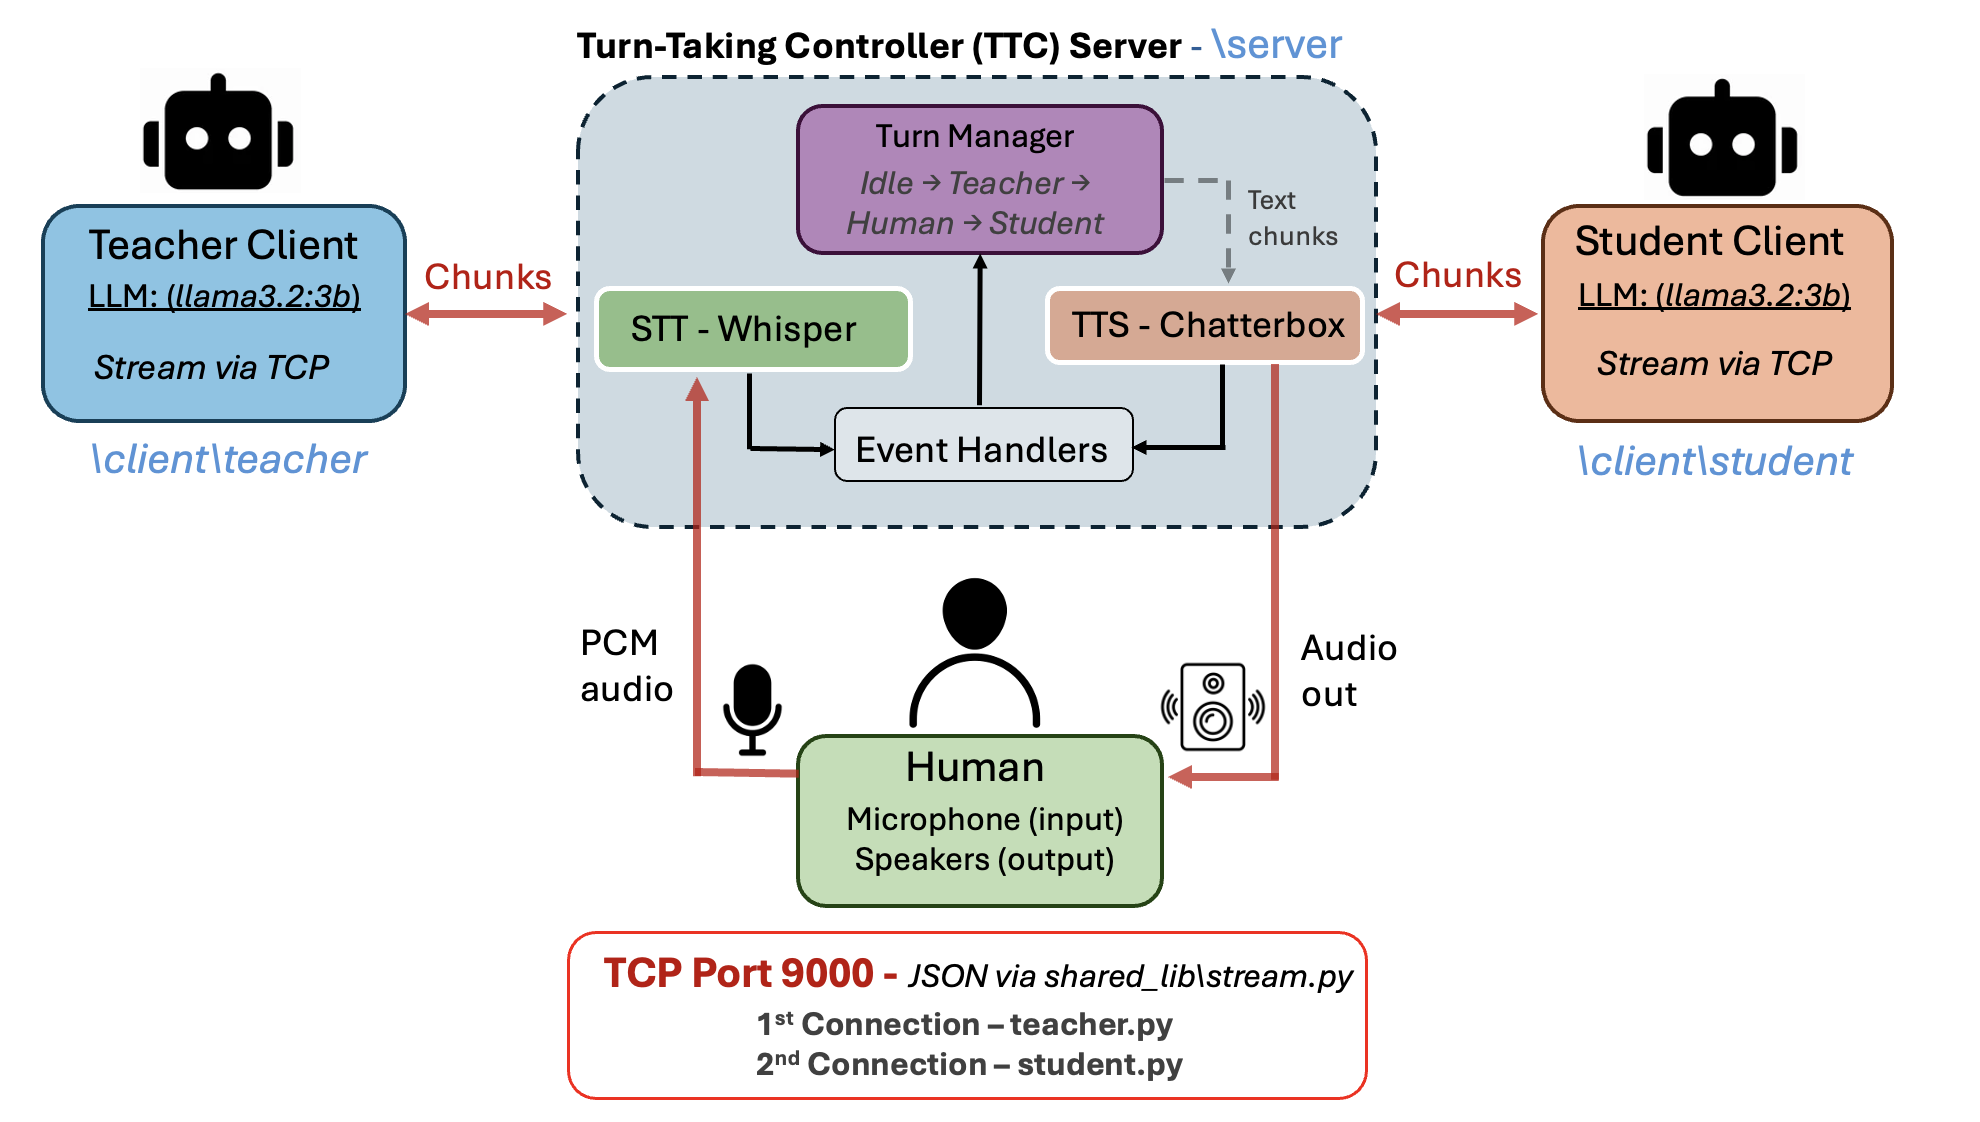
\includegraphics[width=\textwidth]{figures/systemarch.png}
  \caption{Architecture of the proposed system.}
  \label{fig:architecture}
\end{figure*}

\begin{figure*}[t]
  \centering
  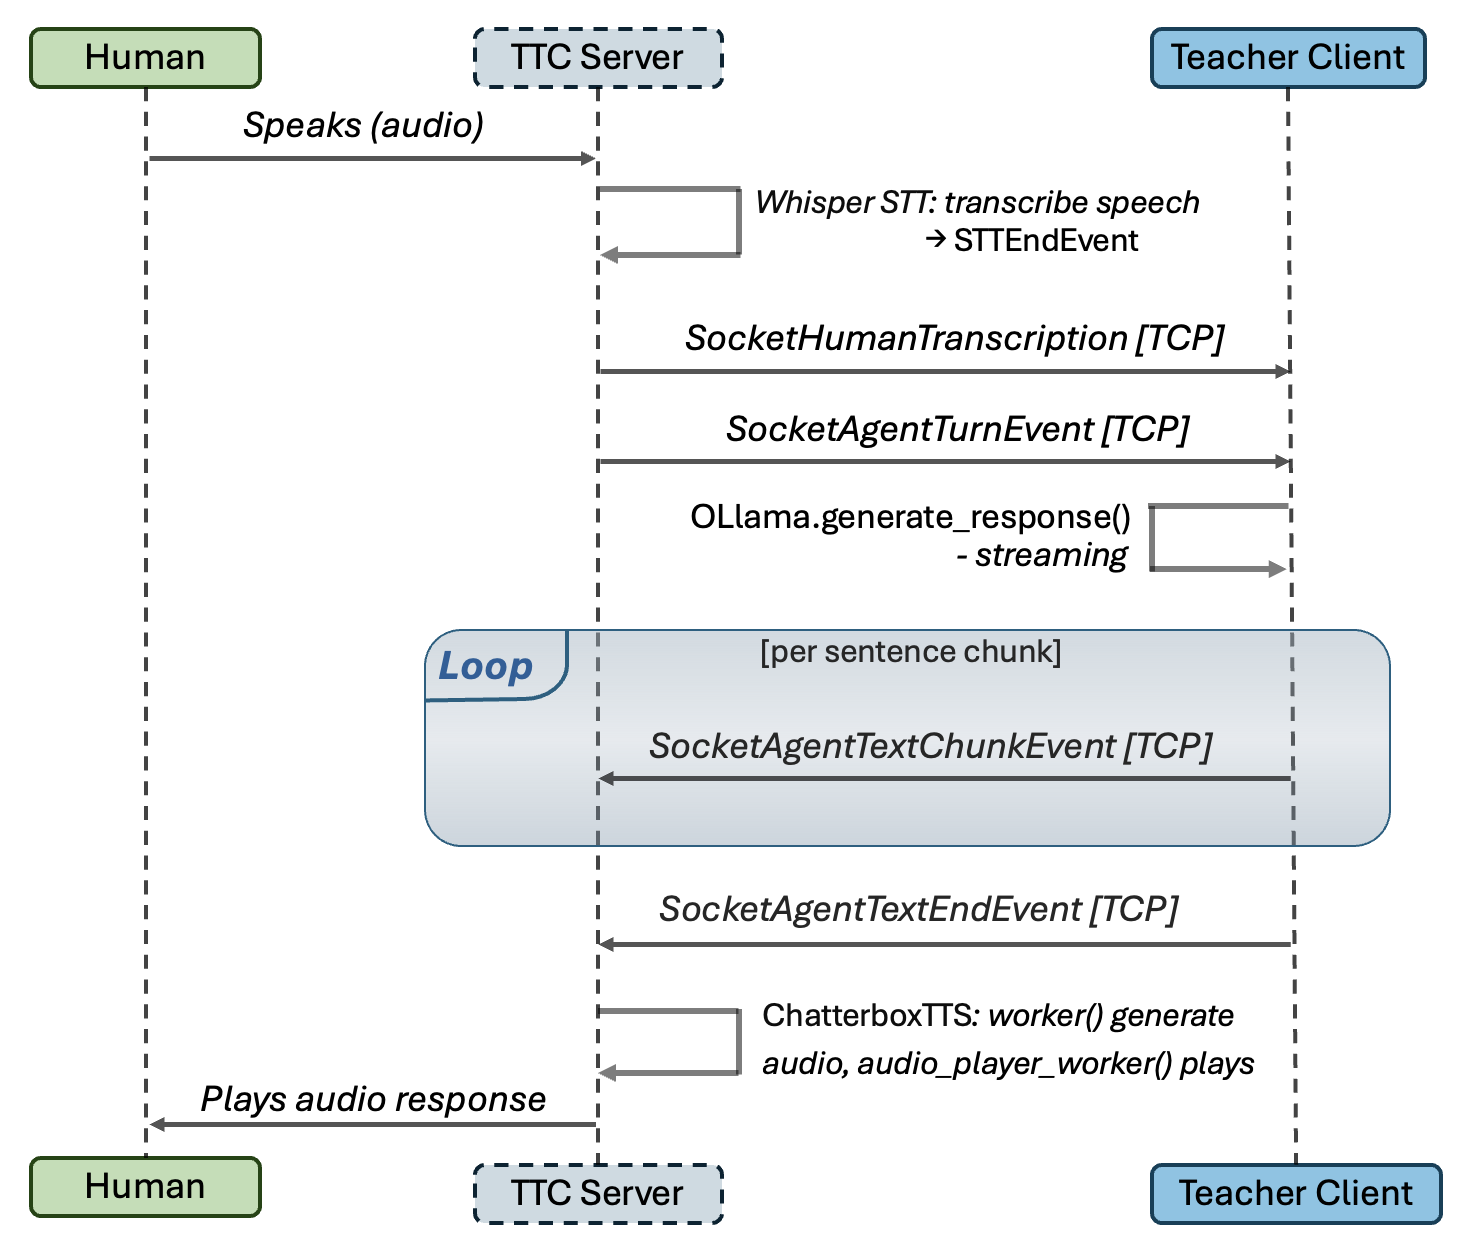
\includegraphics[width=0.72\textwidth]{figures/teacherarch.png}
  \caption{Sequence diagram of the teacher-only interaction workflow (Human, TTC Server, Teacher Client).}
  \label{fig:seq_teacher}
\end{figure*}

\begin{figure*}[t]
  \centering
  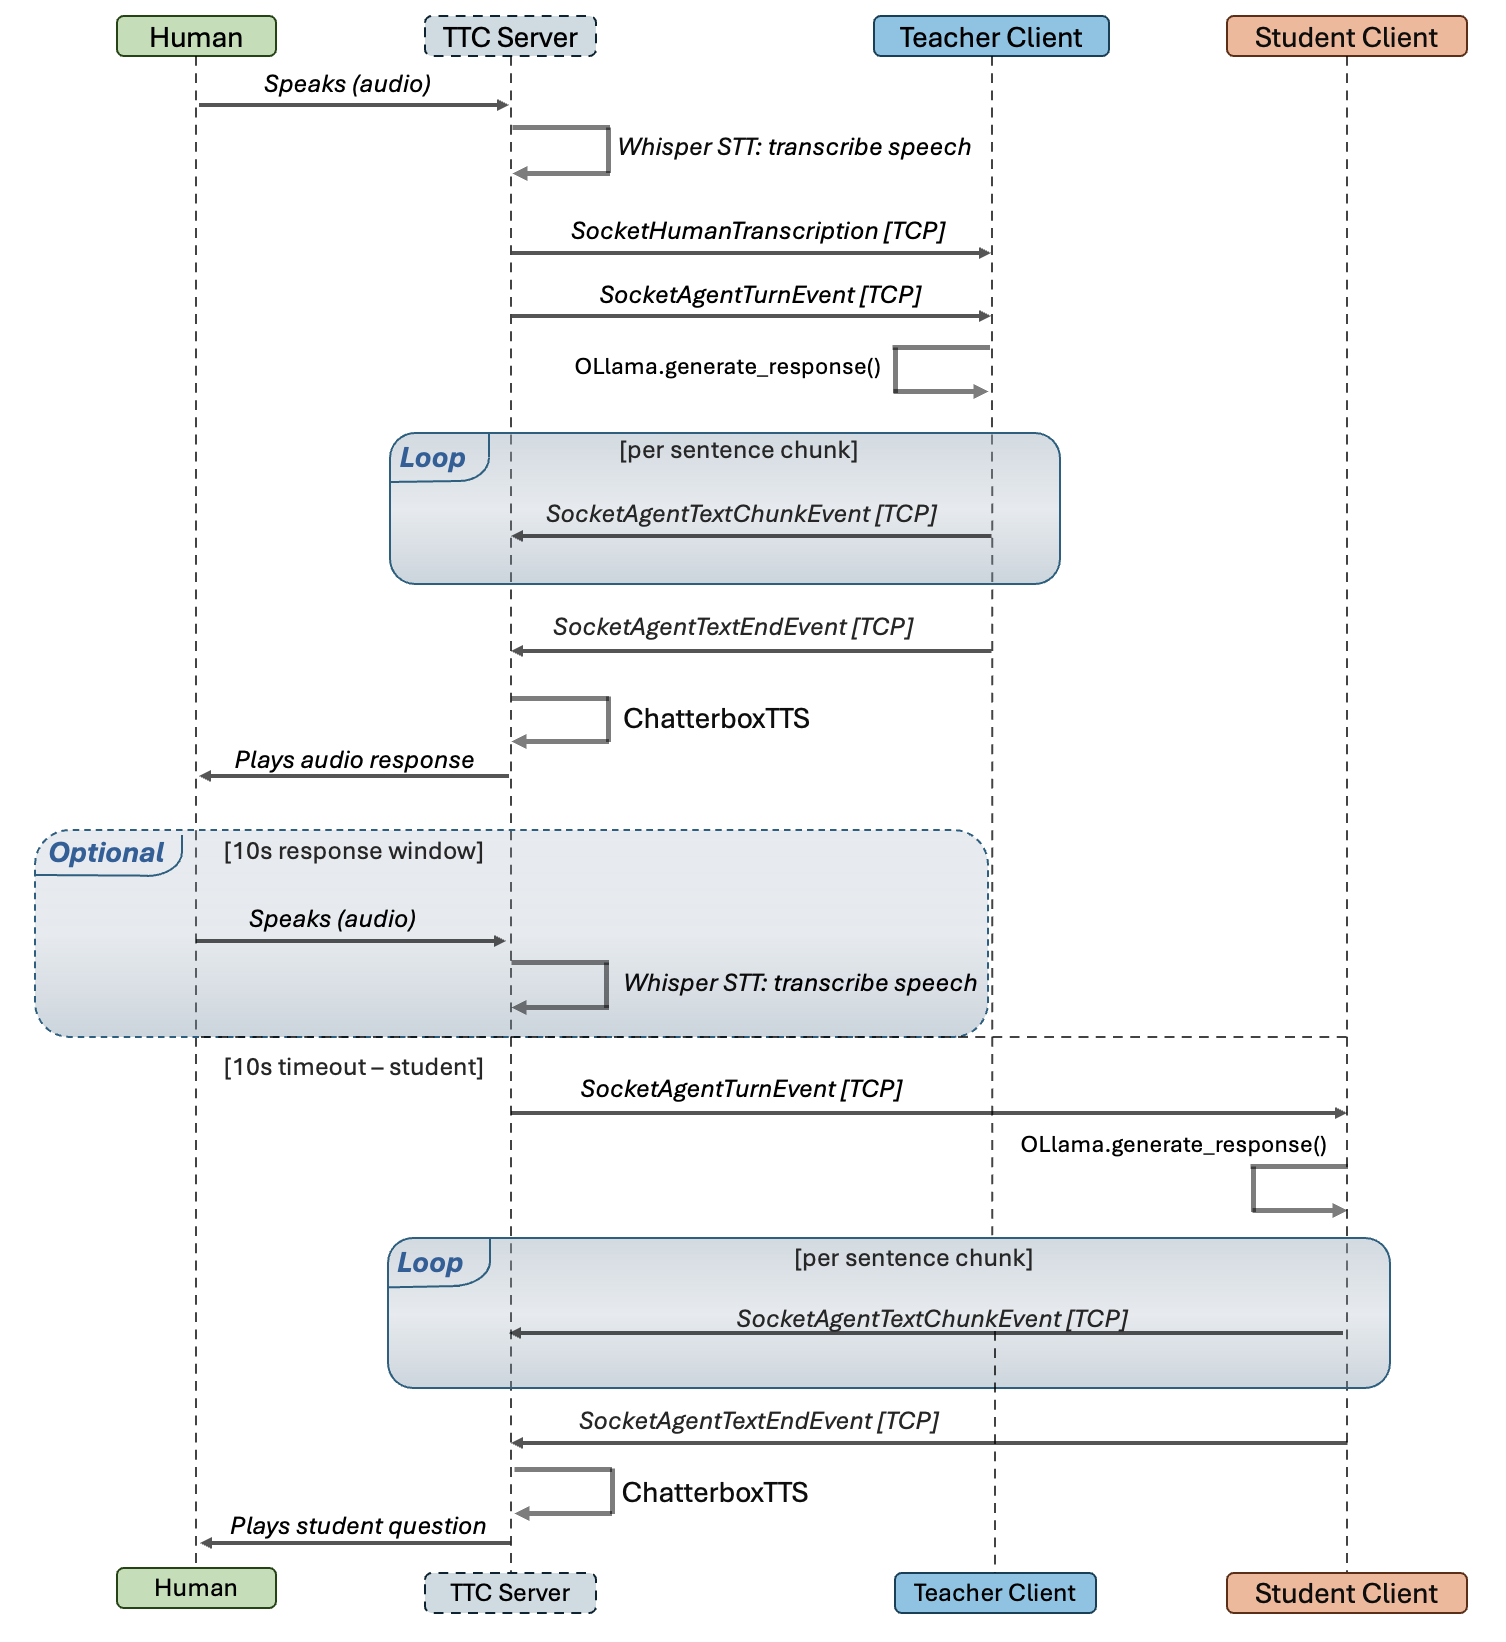
\includegraphics[width=\textwidth]{figures/teacherstudentarch.png}
  \caption{Sequence diagram of the combined teacher--student interaction workflow (Human, TTC Server, Teacher Client, Student Client).}
  \label{fig:seq_combined}
\end{figure*}

% Write architecture overview here.

\subsection{Component A --- [Name]}

\guidance{%
  Describe this component's role in the system, its inputs and outputs,
  and why it was chosen over alternatives. }

% Describe component A.

\subsection{Component B --- [Name]}

% Describe component B.

\subsection{Component C --- [Name]}

% Describe component C (e.g.\ TTS, UI, output module).

\subsection{Design Decisions and Justifications}

\guidance{%
  Summarise the key design trade-offs you made and why. This helps
  demonstrate that the overall design is coherent and well-motivated
  rather than arbitrary.}

% Write design justifications here.



\section{Evaluation}
\label{sec:evaluation}
% ============================================================
% MARKING CRITERION: "Evaluation" [20 marks]
%   - Evaluation methods and metrics discussed thoroughly
%   - Appropriate evaluation plan
%   - Evaluation method clear and sensible
%   - Results / conclusions presented clearly

\guidance{%
  MARKING: This section is worth 20 marks. The marker will check:
  (1) that evaluation methods and metrics are discussed thoroughly,
  (2) that you had an appropriate evaluation plan, (3) that the method
  is clear and sensible, and (4) that results and conclusions are
  presented clearly. Use tables and figures to present results.
  Interpret your results --- do not just state numbers.}

Briefly introduce your evaluation strategy, the scenario(s) tested, and any datasets used.

\subsection{Intrinsic Evaluation}
\label{sec:intrinsic}

\guidance{%
  Describe the intrinsic evaluation: what was measured, what data was
  used (e.g.\ dataset, number of test items), and what metrics were
  applied. Define each metric with a formula if appropriate.}

% Define your metrics:
% \begin{equation}
%   \text{MetricName} = \frac{\text{Numerator}}{\text{Denominator}}
%   \label{eq:metric}
% \end{equation}

\subsubsection{Results}

\guidance{%
  Present intrinsic results clearly in a table. Interpret them ---
  what do they tell you about your system's performance? Compare with
  baselines or prior work where possible.}

\begin{table}[H]
\centering
\small
\begin{tabular}{lcc}
\toprule
\textbf{Metric} & \textbf{Condition A} & \textbf{Condition B} \\
\midrule
Metric 1  & 0.000 & 0.000 \\
Metric 2  & 0.000 & 0.000 \\
Metric 3  & 0.000 & 0.000 \\
\bottomrule
\end{tabular}
\caption{Intrinsic evaluation results.}
\label{tab:intrinsic_results}
\end{table}

% Interpret the results here.


\subsection{Extrinsic Evaluation}
\label{sec:extrinsic}

\guidance{%
  Describe your extrinsic evaluation plan: participant recruitment,
  study procedure, ethical approval, and any measures taken to ensure
  data quality (e.g.\ attention checks, exclusion criteria).}

\subsubsection{Task Performance}

\guidance{%
  Report objective task-level results: task success rate, number of
  turns, slot-filling accuracy, dialogue efficiency, etc.}

% Write task performance results here.

\subsubsection{Behavioural Analysis}

\guidance{%
  If applicable, analyse how the system handled specific user behaviours
  (e.g.\ pauses, self-corrections, interruptions). Present in a table.}

\begin{table}[H]
\centering
\small
\begin{tabular}{lcc}
\toprule
\textbf{Behaviour} & \textbf{Occurrences} & \textbf{Success Rate} \\
\midrule
Behaviour A & 0 & 0\% \\
Behaviour B & 0 & 0\% \\
Behaviour C & 0 & 0\% \\
\bottomrule
\end{tabular}
\caption{Success rates for handling different behaviours.}
\label{tab:behaviour_results}
\end{table}

\subsubsection{Subjective Evaluation}

\guidance{%
  Report questionnaire results. Describe the instrument (e.g.\
  Godspeed, Likert scales), validity checks (KMO, Cronbach's alpha),
  and statistical tests used. Present frequencies and averages with
  figures if possible.}

% Write subjective evaluation results here.

\subsection{Discussion of Results}

\guidance{%
  Tie all evaluation results together. What do the intrinsic and
  extrinsic results tell you collectively? Were there any surprising
  findings? What are the limitations of your evaluation? This is
  where you demonstrate clear and sensible interpretation --- a key
  part of the marking criterion.}

% Write discussion here.


\section{Conclusions}

In conclusion, the proposed project has helped us investigate the effectiveness of vicarious learning in the field of agentic educational learning. Even though the results did not reflect our initial hypothesis in terms of measurable knowledge gains, the Teacher and Student group consistently rated their experience higher across all learning experience dimensions, most notably in engagement and post-session confidence. This is broadly consistent with the vicarious learning hypothesis, suggesting that the presence of a synthetic peer enriches the perceived learning environment even when objective test scores remain relatively equivalent.

The main limitations are the small and informally recruited sample, the ceiling effect on simpler knowledge questions, and the audio-only delivery format. Qualitative feedback highlighted pacing and unnatural silences between turns as the most persistent issues. Future work should focus on a larger controlled study with improved TTS pacing, the incorporation of a visual teaching component, and a more varied Student agent behaviour to strengthen the pedagogical contribution of the synthetic peer.

\subsection{Future Work}

Several directions for future work were identified following the implementation and evaluation of this project.

First, the experiment should be replicated across topics of varying cognitive difficulty, as the relative simplicity of Simpson's Paradox may have contributed to the similar results observed between conditions. Second, end-of-utterance prediction should replace the current fixed response windows, which were the primary source of unnatural silences reported by participants. Third, incorporating a visual teaching component such as slide presentations would more closely replicate a conventional classroom environment. Finally, a larger and more carefully recruited sample would allow for more statistically robust conclusions.



\bibliographystyle{apalike}
\bibliography{references}

\end{multicols}

\newpage
\appendix

\section{Work Assignment}
\label{app:work}

\guidance{%
  Describe each team member's or sub-team's responsibilities. This helps
  the marker understand individual contributions.}

\subsection{Team A: [Names]}
% Describe responsibilities.

\subsection{Team B: [Names]}
% Describe responsibilities.

\subsection{Team C: [Names]}
% Describe responsibilities.

\section{System Design Figures}

\begin{figure*}[t]
  \centering
  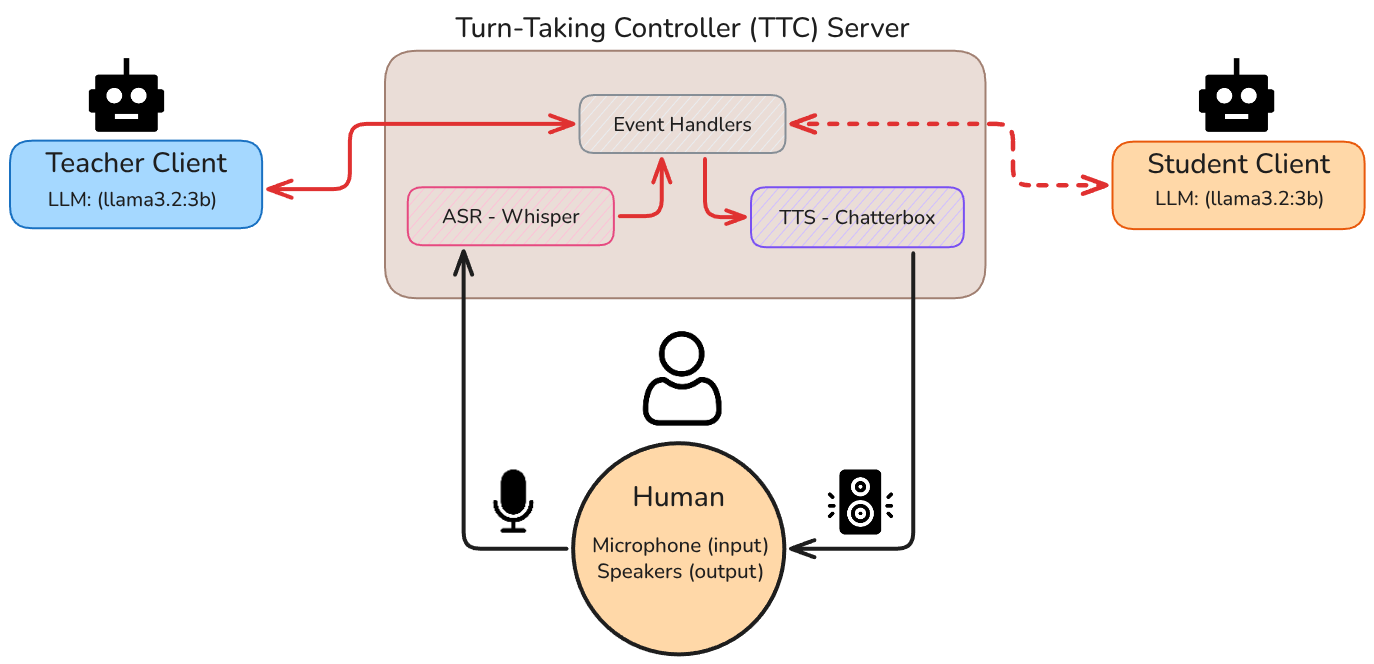
\includegraphics[width=\textwidth]{figures/system.png}
  \caption{Architecture of the proposed system. Boxes represent components, participants are presented as circles, and arrows indicate information flow from source to destination. Boxes with solid filling represent standalone programs, while those with hachured filling represent internal components of a program. Red lines denote events generated by components, while black lines represent raw data. Dashed lines indicate optional connections.}
  \label{fig:architecture}
\end{figure*}


\begin{figure*}[t]
  \centering
  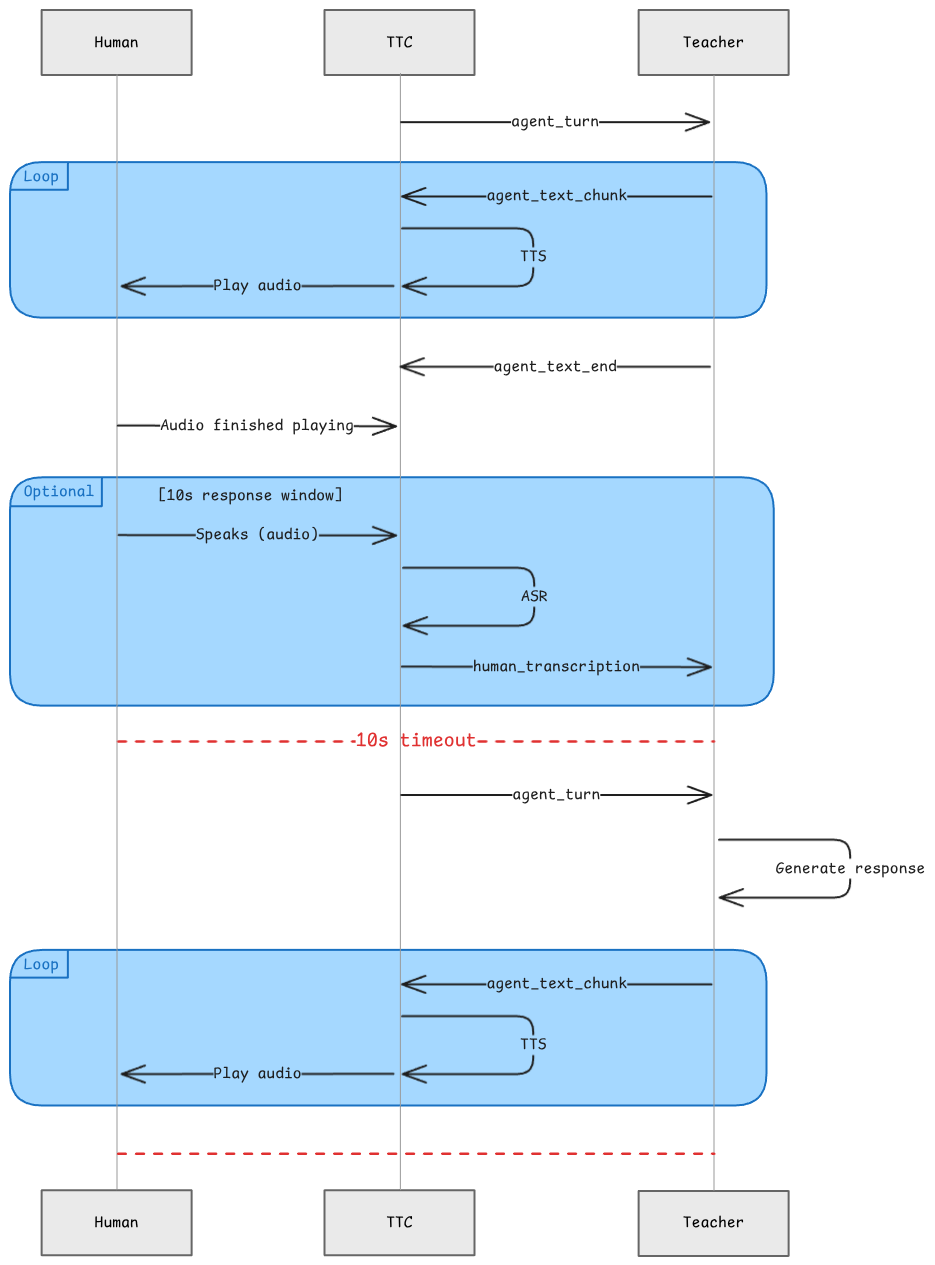
\includegraphics[width=0.72\textwidth]{figures/teacher_seq_diagram.png}
  \caption{Sequence diagram of the teacher-only interaction workflow.}
  \label{fig:seq_teacher}
\end{figure*}

\begin{figure*}[t]
  \centering
  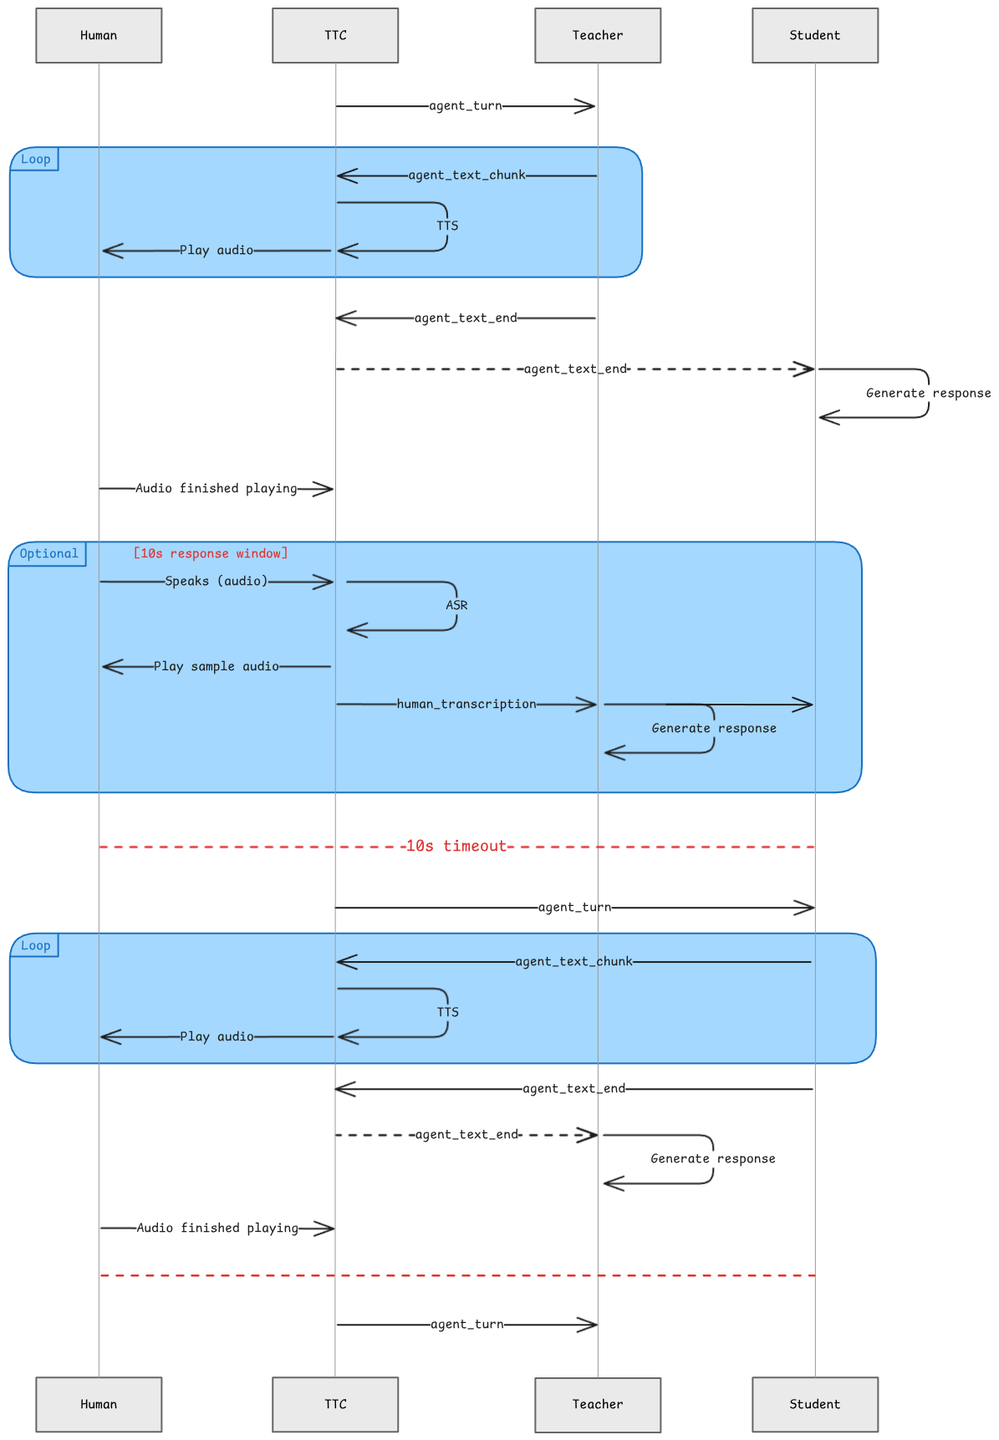
\includegraphics[width=\textwidth]{figures/teacher_student_seq_diagram.png}
  \caption{Sequence diagram of the combined teacher--student interaction workflow.}
  \label{fig:seq_combined}
\end{figure*}

\section{Questionnaire}
\label{app:questionnaire}

\guidance{%
  Include the full questionnaire used in extrinsic evaluation so the
  marker can assess its appropriateness.}

\begin{table}[H]
\centering
\small
\begin{tabular}{llc}
\toprule
\textbf{Aspect} & \textbf{Description} & \textbf{Score} \\
\midrule
Aspect 1 & Low (1) -- High (5) & \\
Aspect 2 & Low (1) -- High (5) & \\
Aspect 3 & Low (1) -- High (5) & \\
\bottomrule
\end{tabular}
\caption{The questionnaire applied in this report.}
\label{tab:questionnaire}
\end{table}


\section{Supplementary Results}
\label{app:supplementary}

\guidance{%
  Include any additional tables, statistical tests (e.g.\ Wilcoxon),
  or detailed breakdowns that support but would clutter the main text.}

% Include supplementary tables here.


\section{Ethical Considerations}
\label{app:ethics}

\guidance{%
  Address: (1) informed consent, (2) data protection and GDPR compliance,
  (3) participant rights (voluntary participation, right to withdraw),
  (4) risk mitigation, and (5) broader considerations such as bias in
  conversational agents.}

% Write ethical considerations here.


\section{Consent Form}
\label{app:consent}

% Include or reference your consent form.
% \begin{figure}[H]
%   \centering
%   \includegraphics[width=0.9\textwidth]{consent_form.png}
%   \caption{Consent form example.}
% \end{figure}


\end{document}
